\documentclass[aps, prc, reprint, amsmath, groupedaddress, nofootinbib]{revtex4-1}
%\usepackage[compat=1.1.0]{tikz-feynman}
\usepackage[utf8]{inputenc}
\usepackage{hyperref}
\usepackage{amsmath}
\usepackage{amssymb}
\usepackage{amsfonts}
\usepackage{tabularx}
\usepackage{booktabs}
\usepackage{graphicx}
\usepackage{color}
\usepackage{multirow}
\usepackage{verbatim}
\usepackage[inline]{enumitem}
\graphicspath{{fig/}}
\definecolor{theblue}{RGB}{0,50,230}
\usepackage{appendix}
\hypersetup{
  colorlinks=true,
  linkcolor=theblue,
  citecolor=theblue,
  urlcolor=theblue
} 
\usepackage[most]{tcolorbox}

\begin{abstract}
Hard probes created in perturbative processes are excellent probes for the study of the hot and dense QCD matter created in relativistic heavy-ion collisions.
Transport approach, allowing for a coupling to an evolving medium with a fluctuating initial condition, has become a powerful tool in this endeavor. 
However, the implementation of the Landau-Pomeranchuk-Migdal (LPM) effect for medium-induced parton branching processes, poses a challenge to semi-classical models: the widely used Boltzmann-type transport equations.  
In this work, we investigated a possible solution, termed the ``modified Boltzmann transport" approach, including a prescription for the running coupling constant.
By fixing two numerical parameters, this approach quantitatively reproduces the medium-induced splitting rates predicted by the next-to-lead-log solution of the AMY equation which is valid in the deep-LPM regime of an infinite medium.
We also found a qualitative agreement of our implementation with calculations in a finite and expanding medium, but future improvements are needed for precision at small path length.
This work will benefit transport model based studies and the usage of these models in the phenomenological extraction of the jet transport coefficient.


\end{abstract}

\begin{document}
\title{A modified-Boltzmann approach for modeling the hot QCD medium-induce splitting vertices in the deep LPM region}
\author{Weiyao Ke}
\author{Yingru Xu}
\author{Steffen A.\ Bass}
\affiliation{Department of Physics, Duke University, Durham, NC 27708-0305}
\date{\today}
\maketitle 

\section{Introduction}
The study of hard probes in relativistic heavy-ion collisions is moving towards the precision era thanks to upcoming experimental upgrades \cite{ATLAS-Collaboration:2012iwa,Abelevetal:2014dna,STAR:upgrade-hf,Adare:2015kwa,CMS:2017dec} as well as theoretical and computational advances that allow for the execution of jet propagations in a realistic Quark-Gluon-Plasma (QGP) medium (including event-by-event fluctuating initial conditions and temperature-dependent transport coefficients) \cite{Wang:1994fx,Zakharov:1996fv,Baier:1996sk,Zakharov:1997uu,Arnold:2002zm,Gyulassy:2003mc,Kovner:2003zj,Jeon:2003gi,CasalderreySolana:2007pr,Djordjevic:2008iz,Bass:2008rv,Schenke:2009gb,Majumder:2009zu,Majumder:2010qh,Armesto:2011ht,Zapp:2011ya,Ovanesyan:2011xy,Kang:2014xsa,Cao:2016gvr,Kauder:2018cdt,Cao:2017zih}. Among the goals for this research is the characterization of the QGP medium in terms of its jet transport coefficients $\hat{q}$.

Transport models are powerful tools where hard probes can be coupled to the realistic time evolution of the medium with an event-by-event fluctuating initial condition. 
However, the numerical implementation of the QCD analog of the Landau-Pomeranchuk-Migdal (LPM) effect, poses a serious challenge to a class of widely used models: the Boltzmann-type transport equation, including the Langevin dynamics.
In a dense medium, multiple scatterings act coherently within the formation time ($\tau_f$) of the medium-induced splitting \cite{PhysRev.103.1811,Wang:1994fx,Zakharov:1996fv,Zakharov:1997uu,Baier:1996kr,Baier:1996sk}, and the rate is significantly reduced compared to an incoherent estimation.
The in-medium splitting becomes an effectively $n$-body to $(n+1)$-body process with a finite extend in space-time compare to the elastic mean-free-path $\lambda_{\textrm{el}} \sim 1/g^2T$.
This feature is particularly difficult to accurately accounted for in a Boltzmann transport equation, where interactions are based on few-body processes whose time scale is much shorter than $\lambda_{\textrm{el}}$, which is true for elastic processes at weak coupling as its duration is proportional to the inverse of Debye mass $1/m_D \sim 1/gT$.
To simplify the problem for splitting processes while still retaining essential qualitative features, different methods have been used in numerical studies \cite{Cao:2013ita,ColemanSmith:2012vr,Xu:2004mz,Zapp:2011ya,Gossiaux:2012cv,Park:thesis}.

In this work we try to identify what approximation we need to make in order to include the LPM effect approximately in a Boltzmann-type transport model, the resultant technique is termed as ``the modified Boltzmann transport" approach in this work. 
As an overview of the method, we first setup a semi-classical transport model with elastic (with both scattering and diffusion) processes and incoherent splitting processes.
The hard partons are transported under the effect of these ``local'' processes.
Then, the LPM suppression and its ``non-locality'' is implemented as a modification to the incoherent splitting processes with both an elastic broadening and a suppression of the splitting probability $\propto \lambda_{\textrm{el}}/\tau_f$ in the leading-logarithmic (LL) picture.
Moreover, we also find a prescription to correct for the logarithmic ambiguity of the LL suppression probability to have the uncertainty of this implementation under a better control.
There is one numerical constant introduced in this approach, but it can be tuned to semi-analytic calculations in an infinite medium limit in the deep LPM regime where the daughter parton's energy is much greater than the temperature \cite{Arnold:2008zu}.
It reasonably describes the medium induced splitting rate for different channels $q\rightarrow q+g$, $g\rightarrow g+g$ and $g\rightarrow q+\bar{q}$, for a wide range of parton energies and at different coupling strengths.
Therefore, the performance of our method is calibrated to theoretical calculations in the deep LPM region.
A tentaive prescription for implementing running coupling is also proposed and has a reasonable agreements with theoretical expectations \cite{Arnold:2009mr}.
This ``calibration to theory'' practice is important for the future application of this transport model to a phenomenological extraction of the jet transport properties from systematic model-to-data comparison, as it is an essential step to reduce the theoretical uncertainty introduced by an approximated modeling of the underlying theory.

The realistic medium that is created heavy-ion collisions is finite with a fast-dropping temperature profile due to longitudinal expansion. 
Therefore, we must investigate if our approach also captures the finite size effect  for branchings with a large formation time compared to the finiteness of the medium.
The interference at the boundary is certainly very complicated and is not built-in in our implementation, however, our approach does display a finite-size effect that qualitatively reproduce the theoretical calculation as function of the path-length and the expansion rate \cite{CaronHuot:2010bp, Baier:1998yf}.
Of course, to achieve a precision level of agreement with the theory as it is in the deep-LPM region, future improvements are definitely needed at small path-length.

This paper is organized as follows. Section \ref{section:Boltzmann} introduces the Linearized Boltzmann plus Langevin transport model using incoherent calculation of parton splitting.
In Section \ref{section:modified-Boltzmann}, we propose an ansatz to modify the aforementioned model in Section \ref{section:Boltzmann} to include the LPM effect.
A next-to-leading-log (NLL) solution in the deep LPM region is used as guidance to determine the form of the ansatz.
Detailed comparisons between the simulation and the NLL solution is found in section \ref{section:results} and appendix \ref{app:tune-spectrum}.
The behavior of this approach in finite and expanding media is investigated in \ref{section:more}.
Finally, \ref{section:summary} is a short summary and outlook.



\section{Semi-classical transport approach with incoherent rates}\label{section:Boltzmann}
In this section, we first build the transport model in the incoherent limit. 
The partonic processes are categorized into elastic (particle number conserving) and inelastic processes (particle number non-conserving). 
The inelastic processes are further divided into parton-splitting and parton-jointing contribution. 
In this section, we shall first proceed using local and incoherent calculation of such processes and will discuss in great detail in the next section on  the inclusion of the LPM effect.

First, we define $Q$ as the momentum transfer between the hard parton and the medium of a process.
To be able to handle both large-$Q$ processes where the medium screening effect is weak, as well as small-$Q$ interactions where medium effect is important,
we separate the interactions into a large-$Q$ (hard mode) section and a small-$Q$ (soft-mode) section.
The former is solved by collision rates calculated with matrix-element computed in the vacuum, and later is solved by diffusion dynamics and diffusion-induced splitting / jointing rates.
The switching scale of the hard/soft modes are chosen to be proportional to the Debye mass square $Q_{\textrm{cut}} = c m_D$, with $c=2$ as default.
One of the many advantages of this separation is avoiding the use of the complicated in-medium propagators, while still achieve an leading order accuracy with a reasonable choice of $Q_{\textrm{cut}}$ \cite{Ghiglieri:2015ala}.

For the diffusion sector, the transverse and longitudinal diffusion constants $\hat{q}_S, \hat{q}_{S,L}$ in a weakly coupled theory with the $Q_{\textrm{cut}}$ dependence have been calculated in \cite{Ghiglieri:2015ala} at leading order,
\begin{eqnarray}
\hat{q}_S = \int_0^{Q_{\textrm{cut}}^2} dq^2 \frac{\alpha_s m_D^2 T}{q^2 (q^2+m_D^2)},
\label{eq:qS} \\
\hat{q}_{S,L} = \int_0^{Q_{\textrm{cut}}^2} dq^2 \frac{\alpha_s m_\infty^2 T}{q^2 (q^2+m_\infty^2)}
\label{eq:qSL}, 
\end{eqnarray}
where the ``$S$'' subscripts reminds us that it only contains soft contributions below $Q_{\textrm{cut}}$.
The drag coefficient determined by the Einstein relation given the transport coefficients,
\begin{eqnarray}
\eta_D = \frac{\hat{q}_{S,L}}{2ET} - \frac{d\hat{q}_{S,L}}{dp^2} - \frac{\hat{q}_{S,L} - \hat{q}_S/2}{p^2}.
\end{eqnarray}
For the large-$Q$ collision sector, the collision rates $R$ for  $2\leftrightarrow2$ and $2\leftrightarrow3$ scatterings are obtained by integrating the vacuum matrix-element over the thermal distribution function $f_0$ of the medium partons, with restriction $Q > Q_{\textrm{cut}}$
\begin{eqnarray}
R_{2\rightarrow n} = \frac{g_i}{2E_1}\int  \frac{d^3p_2}{2E_2(2\pi)^3} f_0(p_2)2\hat{s} \int_{-\hat{s}}^{Q_{\textrm{cut}^2}}\frac{d\sigma}{d\hat{t}}d\hat{t}
\end{eqnarray}
Here $\frac{d\sigma}{d\hat{t}}$ is the differential cross-sections. 
For two-body collisions, we used the standard results but with only $\hat{t}$-channel contribution \cite{RevModPhys.59.465}.
The matrix-elements for the $2\rightarrow 3$ processes are more complicated and we derive them in the limit $k_\perp^2, q_\perp^2 \ll x(1-x)\sqrt{s}$, where $q_\perp$ is the transverse component of $Q$ in the center-of-mass frame, and $k_\perp$ is the transverse momentum of the radiated parton in the final state. 
A list of these matrix-elements can be found in appendix \ref{app:23}.
For the incoherent diffusion-induced splitting rate, we use the expression from \cite{Cao:2017hhk} without the time-dependent coherence factor,
\begin{eqnarray}
R_{1\rightarrow 2} = \int d k_\perp^2 dx \frac{\alpha_s P(x) \hat{q}_S}{2\pi (k_\perp^2 + m_\infty^2)^2}
\end{eqnarray}
where a gluon thermal mass $m_\infty$ is added to screen the divergence.
For the reverse processes $3\rightarrow 2$  and $2\rightarrow 1$ processes, similar reaction rate can be written down.

Combining all these processes, we summarize this hybrid linearized Diffusion plus Boltzmann dyanmics into,
\begin{eqnarray}
\frac{df}{dt} = \mathcal{D}[f] + \mathcal{C}_{1\leftrightarrow 2}[f] + \mathcal{C}_{2\leftrightarrow 2}[f] + \mathcal{C}_{2\leftrightarrow 3}[f].
\end{eqnarray}
The distribution function of the hard parton under goes soft diffusion and diffusion induced-radiation. 
Hard collision with the medium are included as $2\leftrightarrow 2$ and $2\leftrightarrow 3$ collision terms.
This is solved in a particle-based approach where each test particle is updated by,
\begin{eqnarray}
\vec{x}(t+\Delta t) &=& \frac{\vec{p}}{E}\Delta t\\
\vec{p}' &=& \vec{p} - \eta_D \vec{p} \Delta t + \vec{\xi}(t) \Delta t\\
\Delta t\frac{dR(T, \vec{v}, \vec{p}')}{d\vec{p}^3} &\xrightarrow{\textrm{sampling}}& \vec{p}(t+\Delta t).
\end{eqnarray}
Within time step $\Delta t$, the particle first does free transport.
Then, its momentum is updated by the Langevin dynamics with a drag force and a thermal random force to an intermediate state $\vec{p}'$. 
The temporal correlation of the thermal random forces is related to the transport coefficients by,
\begin{eqnarray}
\left\langle\xi_i(t)\xi_j(0)\right\rangle = \delta(t) \left(
\frac{p_i p_j}{p^2}\hat{q}_{S, L} + \left(
\delta_{ij}-\frac{p_i p_j}{p^2}
\right)\frac{\hat{q}_S}{2} 
\right)
\end{eqnarray}
Finally, the particle under goes varies collision channels with the reaction probability $R\Delta t$, and the final states are obtained by sampling the differential collision rate $dR/d\vec{p}^3$.

\section{Modeling LPM effect by a modified transport simulation}\label{section:modified-Boltzmann}
The incoherent transport equation only works for a small window of phase-space where the formation time of the splitting processes is small compared to elastic-mean-free path, which is not the case for energetic splittings and we expect a modification to the above transport approach in this region.

From uncertainty principal, the splitting formation time can be obtained as the inverse of the difference between the final-state energy and the initial-state energy of the splitting system,
\begin{eqnarray}
\tau_f^{-1} \sim \delta E = \frac{[(1-x)\vec{k}_\perp - x\vec{q}_\perp]^2}{2x(1-x)E} 
\label{eq:tauf}
\end{eqnarray}
In the reference frame where the initial parton moves in the $z$-direction, the formation time becomes $\tau_f = 2x(1-x)E/k_\perp^2$.
For high energy splitting, such a formation time can be very large compared to the mean-free-path $\lambda \sim 1/g^2T$ from leading order estimation.
Therefore, the transverse momentum $k_\perp$ can be broadened by multiple scatterings during $\tau_f$.
In an infinite medium, when the number of multiple scatterings $N$ is large (the deep-LPM region), one has on average
\begin{eqnarray}
\left\langle k_\perp^2 \right\rangle \approx \hat{q} \tau_f \label{eq:broaden}
\end{eqnarray}
where $\hat{q} = d \left\langle k_\perp^2 \right\rangle / dt$ is the transport coefficient with contributions from all types of interaction.
Combining Eq. \ref{eq:tauf} and Eq. \ref{eq:broaden}, a crude estimate for the average formation time in an infinite medium is then $\left\langle \tau_f \right\rangle \sim \sqrt{2x(1-x)E/\hat{q}}$.
The multiple interactions within the time has to be resumed and in the leading $\ln(N)$ (leading-logarithmic), the transition rate from interacting with $N$ coherent scattering centers is effectively reduced to the rate induced by with one scattering center. 
The LPM effect strongly modifies the radiation spectrum with a factor $\lambda/\tau_f \sim \sqrt{T/(x(1-x)E)}$ for $\omega, E-\omega \gg T$, where $\omega = xE$ is the energy of the radiated daugther parton.
One also sees that the region where the incoherent transport model is valid is limited to $\lambda \gg \tau_f$, or $\omega, E-\omega \ll T$.
Therefore, quite fundamental modification has to be made to the Boltzmann equation to include splitting processes properly which we shall refer as the so-called ``modified Boltzmann transport" approach.

\subsection{An ansatz for the modified transport}
We start by investigating the leading-order calculation of medium-induced parton splitting in a ``brick" and identify the modification to the Botlzmann formulation.
Here we quote the reorganized formula for medium-induced splitting from \cite{CaronHuot:2010bp},
\begin{eqnarray}
\frac{dP^{a}_{bc}}{d\omega} &=& \int_0^\infty dt \frac{g^2}{\pi E} P_{bc}^{a(0)}(x) \int_t^\infty dt'  F(t', t)
\label{eq:full-theory}
\\
F(t', t) &=& \mathfrak{Re} \int_{{\bf q}', {\bf q}} \frac{i {\bf q}'\cdot {\bf q}}{\delta E} \mathcal{C}(t') K(t', {\bf q}'; t, {\bf q})
\end{eqnarray}
where $P_{bc}^{a(0)}$ is the vacuum splitting function, $\delta E$ the energy difference between initial and final states. 
$\mathcal{C}(t')$ is a Boltzmann-like collision operator such that,
\begin{eqnarray}
\mathcal{C}[f] = \int_{\bf q} g^2\mathcal{A}(q_\perp^2)
&&\left\{  \frac{C_b+C_c-C_a}{2}\left(f_{\bf p}-f_{{\bf p}-{\bf q}}\right) \right.\\\nonumber
 +&&    \frac{C_a+C_c-C_b}{2}\left(f_{\bf p}-f_{{\bf p}+x{\bf q}}\right) \\\nonumber
+&&  \left. \frac{C_a+C_b-C_c}{2}\left(f_{\bf p}-f_{{\bf p}+(1-x){\bf q}}\right)\right\},
\end{eqnarray}
where $C_i$ is the color factor of each parton. 
The collision kernel is given by \cite{Aurenche:2002pd},
\begin{eqnarray}
\mathcal{A}(q_\perp^2) = \frac{m_D^2 T}{q^2\left(m_D^2+q^2\right)}
\end{eqnarray}
Finally, $K(t', {\bf q}'; t, {\bf q})$ is the propagator of the transverse  Hamiltonian $\hat{H} = \delta E - i\mathcal{C}$ in the momentum representation.
This rather compact result is actually hard to implement in a Boltzmann formulation, because of the double time integral that signatures the quantum transition.
Moreover, the branching probability generally dependents on the temperature and flow velocity profiles of the medium, making it a computationally heavy task when coupled to dynamical evolving and fluctuating medium.

Our approximation towards a modified Boltzmann transport formulation starts by replacing the effect of the temporal correlator $F(t',t)$ with a simple ansatz,
\begin{eqnarray}
F(t', t) \rightarrow \frac{1}{N}\sum_{i=1}^N \frac{b}{\tau_i(t)} \delta(t-t'- a \tau_i(t))
\end{eqnarray}
Here the function $F(t', t)$ is approximated by an ensemble ($N$) of copies of the branching system $a\rightarrow b+c$.
Each copy ``$i$" evolves with the incoherent transport equation, and there is certain probability for this copy to have a formation time $\tau_i$ at time $t$ during the evolution.
The delta function expresses that the branching that start at time $t'$  is thought to be formed at time $t+a\tau_f$.
The additional factor $b/\tau_f$ corrects for that the probability for a branching to happen is different from the incoherent probability as given by the leading-log pivture.
This ansatz of representing a correlation function using information at $t$ and $t'$ of an ensemble of particles follows the same spirit in the Monte-Carlo solver of the traditional Boltzmann equation, where the distribution function is represented by an ensemble of particles at time $t$.
This is indeed a crude approximation of $F(t', t)$, and its validity has to be examined by comparing its prediction with the theoretical calculations.
Finally, $a$ and $b$ are dimensionless factors whose forms shall be determined later and will be tuned to achieve an optimal level of agreement to theoretical calculations.

With such an ansatz, the medium-induced splitting probability reduces to,
\begin{eqnarray}
\nonumber
\frac{dP^{a}_{bc}}{d\omega} &=& \int_0^\infty dt \frac{g^2 P_{bc}^{a(0)}}{\pi E\tilde{\lambda}(t)} \int_t^\infty dt' \frac{\tilde{\lambda}(t)}{N}\sum_{i=1}^N \frac{b}{\tau_i(t)} \delta(t-t'- a \tau_i(t)) \\
&=& \frac{1}{N}\sum_{i=1}^N\int_0^\infty dt \frac{dR_{\textrm{incoh}}(t)}{d\omega} \times \left.\frac{ab\tilde{\lambda}(t)}{\tau_f(t',t)}\right|_{t'=t+a\tau_f}
\end{eqnarray}
where we have divided and multiplied back an effective mean-free-path $\tilde{\lambda} = m_D^2/\hat{q}_g$ so that we may interpret the quantity immediately after the $dt$ integral as an incoherent splitting rate $R_{\textrm{incoh}}$.
Now it is clear how we can modify the standard Botlzmann transport to approximately include the LPM effect,
\begin{enumerate}
\item Evolve each parton by solving the collision rate equation with incoherent rate from $t$ to $t+\Delta t$.
\item The daughter partons from splittings are not immediately treated as independent (``preformed"). They are evolved together with the mother parton. Preformed partons only undergoes elastic collisions (the mother parton can keep splitting).
\item Recalculate formation time $\tau_f$ after each time step.
\item Repeat steps 1 to 3 until $t' > t + a\tau_f$ is satisfied. 
Then, accept this splitting process with probability 
\begin{eqnarray}
p = \frac{ab\tilde{\lambda}(t)}{\tau_f}
\label{eq:rejection}
\end{eqnarray}
Accepted splittings will be treated as independent objects from time $t'$. and will interact through both elastic and inelastic channels.
Rejected splittings are dropped and do not cause physical effect.
\end{enumerate} 
A key step is a self-consistent determination of the formation time as described in step 4, which in a static medium, results in an averaged formation time scaling like $\left\langle\tau_f\right\rangle \propto \sqrt{\omega/\hat{q}}$.
This procedure also generalizes to medium with evolving temperature profile.
This iterative procedure was first developed and implemented by \cite{Zapp:2011ya}.

Such an ansatz only captures the qualitative behavior of the LPM effect in a large medium. 
To make it more useful, we compare it to theory calculations in an infinite medium in the following subsection and determine the forms of $a$ and $b$.

\subsection{Matching the ansatz to semi-analytic calculation}
The equation \ref{eq:full-theory} in an infinite medium limit is known as the AMY formalisim \cite{Arnold:2002ja,Arnold:2002zm,Arnold:2003zc},
\begin{eqnarray}\label{eq:AMY-1}
\nonumber
\frac{dP_{a\rightarrow bc}}{dt dx} &=& \frac{1}{2E\nu_a} \frac{\alpha_s d_a P_{a\rightarrow bc}(x)}{2x^2(1-x)^2}\int\frac{d^2\vec{h}}{(2\pi)^2}2\vec{h}\cdot \mathfrak{Re} \vec{F}
\end{eqnarray}
where we have dropped the Bose enhancement and the Pauli blocking factors from the original formula.
The vector function $\vec{F}(\vec{h}; p, x)$ satisfies the following equation,
\begin{eqnarray}\label{eq:AMY-2}
\nonumber
2\vec{h} &=& i\frac{h^2 \vec{F}(\vec{h})}{p^3 2x(1-x)} + g^2 \mathcal{C}[\vec{F}]
\end{eqnarray} 
The exact solution can be solved numerically and applied to transport modeling \cite{Jeon:2003gi,Schenke:2009gb}, but we shall use approximated semi-analytic solutions obtained by the author of \cite{Arnold:2008zu}.
These approximated solutions were obtained at the leading-log (LL) and next-to-leading-log (NLL)accuracy, and the NLL solution was shown to be a good approximation of the numerical results in the deep LPM regime $\omega \gg T$.

At leading-log (LL) order, a small-$q$ expansion was performed to obtained a diffusion approximation to $\mathcal{C}$ below a certain cut-off $q<Q_0$.
The resulting leading-log solution is \cite{Arnold:2008zu},
\begin{eqnarray}\label{eq:AMY-LL}
\frac{dP_{bc}^{a,\textrm{LL}}}{dt dx} &=& \frac{\alpha_s P_{bc}^{a(0)}}{\pi\sqrt{2}}
\sqrt{\frac{\hat{q}_3(x, Q_0^2)}{2x(1-x)E}}
\end{eqnarray}
Where the $\hat{q}_3$ is defined as an effective transport parameter for conveniences,
\begin{eqnarray}
\hat{q}_3(x, Q_0^2) &=& \alpha_s T m_D^2 \ln\left(1+\frac{Q_0^2}{m_D^2}\right) C_{abc}(x).\label{eq:qhat3}
\end{eqnarray}
And it depends on the color structure of the splitting,
\begin{eqnarray}
C_{abc}(x) &=&  \frac{C_b+C_c-C_a}{2} + x^2 \frac{C_a+C_c-C_b}{2} \\\nonumber
&+& (1-x)^2\frac{C_a+C_b-C_c}{2}
\end{eqnarray}
Comparing the leading-log formula to the simple ansatz in the modified Boltzmann approach, there is indeed a piece that plays the row of inverse formation time $\langle\tau_f^{-1}\rangle \sim \sqrt{\hat{q}_3 / 2x(1-x)E}$. 
However, the effective $\hat{q}_3$ is differed by an $x$-dependent color factor $C_{abc}$ from the broadening expected from one daughter parton re-scattering that is implemented in our algorithm.
This is improved by defining an $x$-dependent $a$ parameter,
\begin{eqnarray}
a \rightarrow a_{abc}(x) = \frac{C_A}{C_{abc}(x)}
\end{eqnarray}

The LL solution is ambiguous upto an unknown cut-off $Q_0$  through $\hat{q}_3$, coming from integrating the perturbative tail of the collision kernel.
In the Boltzmann approach, the large-$Q$ matrix-element are always integrated upto the maximum transfer bounded by the center-of-mass energy $\sqrt{s}$. Therefore, the average $Q_0^2$ is $\langle\hat{s}\rangle = 6ET$.
The $Q_0$ ambiguity can be improved by going to the NLL order, where the contribution of the collision kernel above $Q_0$ is treated as a pertrubation on top of the LL solution.
This ``single-hard" correction to the ``multiple-soft" approximation is also recently studied in \cite{Mehtar-Tani:2019tvy} in the BDMPS framework.
And the NLL result is the LL solution replacing the unknown $Q_0$ with $Q_1$,
\begin{eqnarray}
Q_1^2  \approx \sqrt{\omega \hat{q}} \approx \sqrt{\omega \alpha_s C_R m_D^2 T \ln\frac{Q_0^2}{m_D^2}}
\label{eq:Q1}
\end{eqnarray}
or a self-consistent determination as in \cite{Arnold:2008zu},
\begin{eqnarray}
Q_1^2 &=& \sqrt{2 x (1-x) E \alpha_s T m_D^2}\\\nonumber
&\times & \left(
\frac{C_b+C_c-C_a}{2}\ln\frac{2\xi Q_1^2}{m_D^2} \right.\\\nonumber 
&+& \frac{C_a+C_c-C_b}{2} x^2 \ln\frac{2\xi Q_1^2}{x^2 m_D^2} \\\nonumber 
&+& \left.\frac{C_a+C_b-C_c}{2} (1-x)^2 \ln\frac{2\xi Q_1^2}{(1-x)^2 m_D^2} \right)^{1/2}
\label{eq:Q1-sf}
\end{eqnarray}
Comparing this NLL result with the modified Boltzmann implementation, the correct scale $\sqrt{\omega \hat{q}}$ is smaller than the upper bound of matrix-element integration $Q_0^2 \approx 6ET$ from the matrix-element integration.
We absorbed this effect into a scale-dependent $b$ parameter to correct the na\"ive choice of $Q_0 \sim \sqrt{6ET}$ that comes from the matrix-element integration,
\begin{eqnarray}
b &=& 0.75\sqrt{\frac{\ln(\hat{Q}_1^2 )}{\ln(\hat{Q}_0^2 )}}.
\label{eq:NLL-b}
\end{eqnarray}
with $\hat{Q}_1^2$ and $\hat{Q}_0^2$ given by,
\begin{eqnarray}
\hat{Q}_1^2 &=& 1 + \frac{\sqrt{\omega\hat{q}}}{m_D^2} \approx 1 + \frac{\tau_f}{\tilde{\lambda}}; 
\hat{Q}_0^2 = 1 + \frac{6ET}{m_D^2}
\end{eqnarray}
The prefactor $0.75$ was tuned when comparing the modified-Boltzmann simulation to the NLL solutions in the next section, and will be the same for the rest of the paper.

As a remark, this logarithmic correction comes from the $q^2 dq^2 /q^4$ integration of the collision kernel at large-$q^2$.
Therefore, if one assumes and implements certain collision kernel that vanishes sufficiently fast at large-$q$, this logarithm factor in $b$ is unnecessary. 

\subsection{Implement running of $\alpha_s$}\label{section:running}
Finally, we discuss the prescription of the running coupling constant in the modified Boltzmann approach.
We used the leading order running coupling constant with $n_f = 3$ and $\Lambda = 0.2$ GeV, 
\begin{eqnarray}
\alpha_s(Q^2) = \frac{4\pi}{9\ln\left(Q^2/\Lambda^2\right)}
\end{eqnarray}
To avoid the pole when $Q$ approaches the non-perturbative scale, we introduce a cut-off using a medium scale $Q_{\textrm{med}} = \pi T$. 
Therefore the actual coupling constant is $\alpha_s(\max\{Q, Q_{\textrm{med}}\})$.
Following the prescription described in \cite{Arnold:2008zu}, the coupling constant associated to the collision kernel $\mathcal{C}$ are evaluated at $q_\perp^2$ and the resulting $\hat{q}$ can be integrated approximately to get the running version of the Eq. \ref{eq:qhat3},
\begin{eqnarray}
\hat{q}_3^{\textrm{running}} \approx \frac{4\pi}{9}\left(g^2(m_D^2) - g^2(Q_0^2)\right) 1.27 T^3 C_{abc}(x)
\label{eq:q3running}
\end{eqnarray}
Where the scale $Q_0$ is of order $m_D [E/T \ln(E/T)]^{1/4}$.
And the scale of the $\alpha_s$ associated to the splitting  vertex in equation \ref{eq:AMY-LL} is chosen at the typical transverse momentum $k_\perp^2 \sim \sqrt{2x(1-x)E\hat{q}_3}$.

In the modified Boltzmann approach, such a running coupling prescription is straightforward for the elastic part.
The transport coefficients $\hat{q}_S$ and $\hat{q}_{S, L}$ in Eq. \ref{eq:qS} and Eq. \ref{eq:qSL} for the diffusion sector should be integrated using the running coupling constant.
The $\alpha_s$ associated to the $2\rightarrow 2$ scattering matrix-elements (including the ones that appears in the $2\rightarrow 3$ matrix-elements) are evaluated at the $t$-channel momentum transfer squared.
The scale $k_\perp^2$ for the splitting vertex coupling requires an additional treatment.
In the presence of the LPM effect, $k_\perp$ comes from the summation over multiple scatterings within the formation time,
\begin{eqnarray}\label{eq:kTn}
\vec{k}_{\perp, t_0+\tau_f}^2 = \left(\vec{k}_{\perp,t_0}+\vec{q}_1+\cdots+\vec{q}_n\right)^2.
\end{eqnarray} 
However, the initial splitting processes are generated using incoherent processes with the coupling evaluated at $\vec{k}_{\perp}^2(t_0)$.
This is on average $\sqrt{\omega/T}$ times smaller than $\vec{k}_{\perp}^2(t_0+\tau_f)$ in the deep LPM region.
Therefore the effective coupling after multiple scattering is smaller than the one we used in incoherent calculation and allows for a rejection implementation by modifying the acceptance probability $p$ in Eq. \ref{eq:rejection} to
\begin{eqnarray}
p^{\textrm{running}} = p\times \frac{\alpha_s(k_{\perp,t_0+\tau_f}^2)}{\alpha_s(k_{\perp,t_0}^2)}.
\end{eqnarray}
This final step completes the inclusion of running coupling effect in the modified Boltzmann approach.

\section{results}\label{section:results}
\begin{figure}
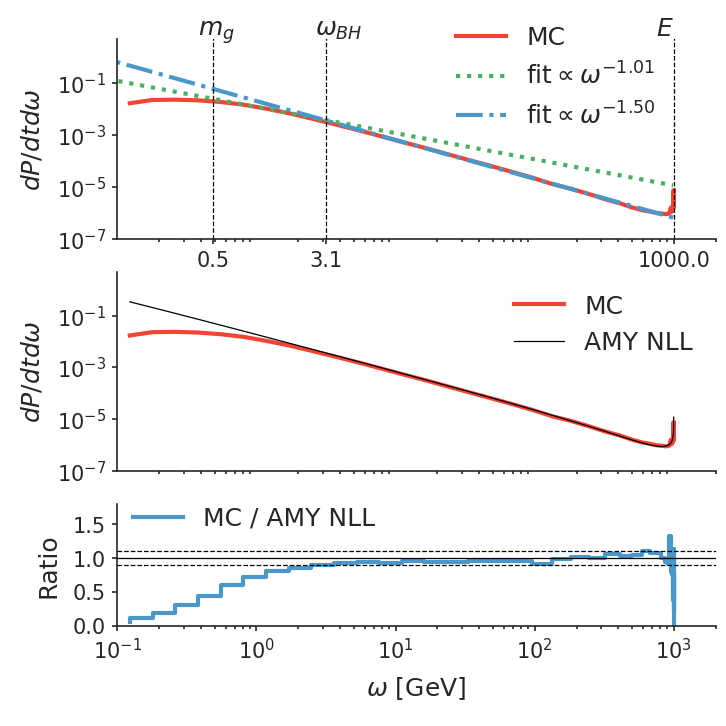
\includegraphics[width=\columnwidth]{spectrum.png}
\caption{The $q\rightarrow q+g$ splitting rate in an infinite medium from a quark with $E=1$ TeV,and a coupling constant $\alpha_s = 0.1$. The top plot shows the simulated spectrum $dR/d\omega$ (red-dashed line) and power law fit (green-dotted and blue-dash-dotted lines) in different gluon energy regions, separated by energy scales $\omega_{BH}\approx 2\pi T$. The middle plot compares to the simulation to NLL solution to the AMY equation, and the ratio is shown in the bottom plot}
\label{fig:spectrum}
\end{figure}

\begin{figure}
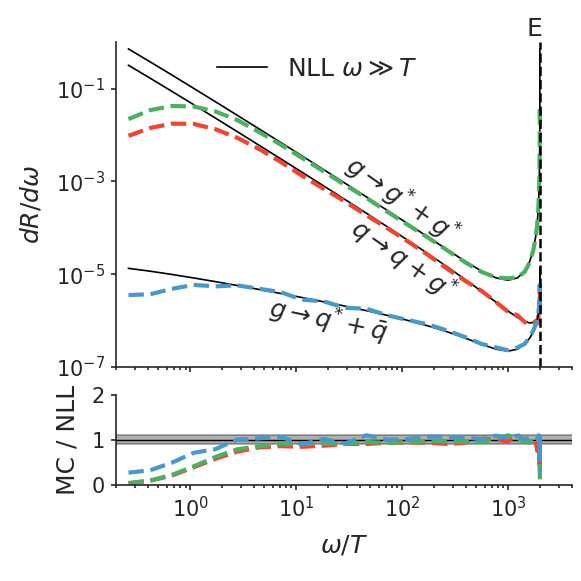
\includegraphics[width=\columnwidth]{channel_rate.png}
\caption{The splitting rate of $q\rightarrow q+g^*$, $g\rightarrow g+g^*$, and $g\rightarrow q^* + \bar{q}$ as a function of the parton energy labeled by the star. The mother parton with $E=1$ TeV evolves inside an infinite medium with $T=0.5$ GeV. The simulations (thick dashed lines) are compared to the NLL solutions (thin solid lines).}
\label{fig:channel_rate}
\end{figure}

\begin{figure}
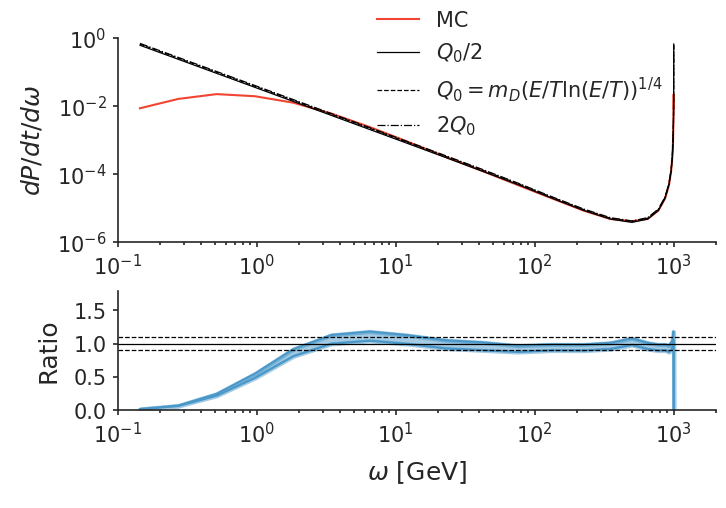
\includegraphics[width=\columnwidth]{running.png}
\caption{Top plot: comparison of modified Boltzmann simulation with the NLL solution  with running coupling.
Three initial guesses of the 
The ratio between simulation and theory is shown in the bottom plot.}
\label{fig:running}
\end{figure}

In this section, we compare the splitting rate $dR/d\omega$ that comes out of the modified Boltzmann approach simulation to the NLL approximation in the infinite medium limit.

The differential rate in an infinite medium $dR/d\omega$ is shown in Figure \ref{fig:spectrum} for a 1 TeV quark splitting into a gluon and a quark.
The temperature of the medium is $T=0.5$ GeV, and a rather small coupling constant $\alpha_s = 0.1$.
Please also refer to Appendix \ref{app:tune-spectrum} for a full comparison varying both the parton energy and the coupling constant.
The horizontal axis is the radiated gluon energy.
In the upper plot, we divided the spectrum into different regions by the gluon thermal mass $m_\infty$ and an estimated Bethe-Heitler energy $\lambda_g m_D^2 \sim 2\pi T$.
The spectrum with above the is suppressed due the use of a finite mass.
In the Bethe-Heitler region $\omega < 2\pi T$, the spectrum scales like $\omega^{-1}$ which comes from the incoherent radiation rate.
In the LPM region $2\pi T < \omega < E$, the spectrum is dominated by coherent multiple scatterings and scales like $\omega^{-3/2}$.
The power-law fits in each domain are very close to the expected scaling.
In the middle plot, we compare the simulation to the NLL solution with self-consistent $Q_1^2$ from Eq. \ref{eq:Q1-sf}. 
The ratio between the two is shown in the bottom plot.
There is a good agreement in the LPM region between the simulation and the theory calculation, which we have used as guidance in developing our Monte-Carlo approach.

A comparison of the other channels $g\rightarrow g+g$ and $g\rightarrow q+\bar{q}$ to the theory calculations are shown in Figure \ref{fig:channel_rate}.
For the splitting parton energy much greater than temperature $\omega > 10 T$, the simulation agrees well with the theory. 

Finally, we compare the running coupling calculation with the theory curve in Fig. \ref{fig:running} for the $g\rightarrow g+g$ channel.
The theory curves (black lines) are obtained combining Eq. \ref{eq:AMY-LL} and Eq. \ref{eq:q3running}.
Different line styles correspond to the variation of the $Q_0$ value around an initial guess $m_D (E/T \ln(E/T) )^{1/4}$ by a factor of $2$ above and below.
For this 1 TeV parton, the scale $Q_0$ is actually very large and the running of $\alpha_s$ is rather slow, which explains the theory curve is not very sensitive to a factor of $4$ change in $Q_0$.
The simulation was performed using the running coupling prescription described in Section \ref{section:running}.
The overall shape of the spectrum in the deep LPM region is again well described by the modified Boltzmann simulation. 


\section{Towards phenomenological applications}\label{section:more}
In the previous section, we have shown that the modified Boltzmann equation simulation has a good agreement with the theoretical calculation for parton splitting in the LPM regime in an infinite medium.
Towards future phenomenological application, we would like to investigate a few more complex scenarios involving finite and expanding medium.

\subsection{Results in a finite medium}
For calculation in a finite medium, there is an intricate interference pattern near the boundary which requires solving the original equation using a finite medium temperature profile. 
Or for the case of a thin medium, such effect can be analyzed order by order in the ``opacity ($L/\lambda$) expansion". 
One important effect in a finite medium is the path-length dependent radiation rate for $L \lesssim \tau_f$, which is important for heavy-ion collisions phenomenology, considering the formation time of very energetic splitting can be comparable to the size of the QGP fireball.
Though the modified Boltzmann approach has been constructed to mimic the rate $dR/d\omega$ in the infinite medium limit, and does not recover the exact form of spectrum for a finite medium, it still predicts an $L$-dependent rate and we would like to check whether it is significantly different from the theory expectation.
The origination of the path-length dependence in the modified Boltzmann approach is that the gluons sampled at $t=t_0$ are not considered as independent objects until $t = t_0+\tau_f$, meaning the splittings at time $t$ is initiated by inelastic processes at $t-\tau_f$.
As a result, in a semi-infinite medium with a step function like temperature profile, 
\begin{eqnarray}
T = \begin{cases}
0 , z<0\\
T_0, z>0
\end{cases}
\end{eqnarray}
there are no scattering centers at $L-\tau_f<0$ and thus introduces a reduction in the radiation rate for small path-length.

\begin{figure}
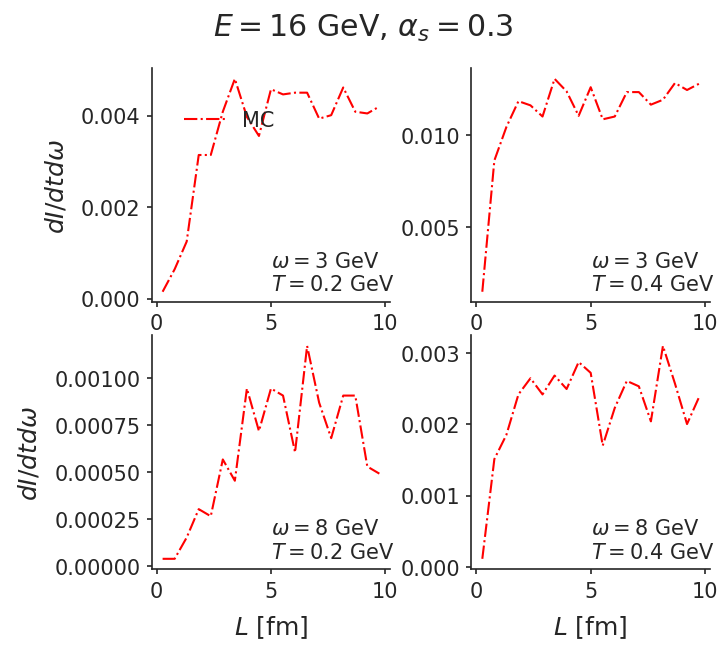
\includegraphics[width=\columnwidth]{spectrum_L.png}
\caption{Comparison of the path-length dependent rate $dR/d\omega$ from the simulation using $\alpha_s = 0.3$ to the theoretical calculation for splitting $q\rightarrow q+g$ \cite{CaronHuot:2010bp}. The quark energy is $16$ GeV.}
\label{fig:spectra-L-alphas=0.3}
\end{figure}

In Figure \ref{fig:spectra-L-alphas=0.3}, the $q\rightarrow q+g$ rate simulated in a semi-infinite medium is compared to the full calculations obtained in \cite{CaronHuot:2010bp}.
The energy of the quark is 16 GeV, and $\alpha_s = 0.3$.
The medium temperature of the left and the right columns are 0.2 GeV and 0.4 GeV respectively.
Top and bottom rows show the differential rates for the emitted gluon  energy $\omega = 3$ GeV and $\omega = 8$ GeV \footnote{In practical simulation, the rate are obtained by counting gluons within a finite energy range $\omega\pm 0.5$ GeV}.
The different rate $dR/d\omega$ are plotted as function of the path length $L$.
It is evident that theoretical rates (black solid lines) first grow approximately linearly with $L$ and then bend over to transit to $L$-independent ones.
The simulation describes the large $L$ limit well and also approximately captures the point at which the transition happens.
But there are systematic deviations compared to the theory at small path-length.
Therefore it will be of great interest to improve to the current simulation approach at small path-length in the future. 
For example, one possible solution would be using the results from the opacity expansion in the simulation for those splittings that happened close to the boundary and developing matching conditions to the approach we used for the deep LPM regime.

\subsection{Results in an expanding medium}
\begin{figure}
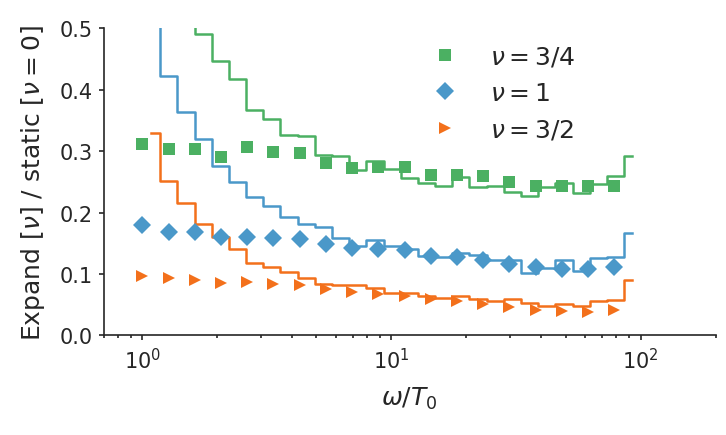
\includegraphics[width=\columnwidth]{spectrum_Bjorken.png}
\caption{The ratios of induced splitting rate in expanding medium to that of a stat medium, with expansion parameter $\nu = 3/4, 1$, and $3/2$. The analytic results are shown in solid lines and simulations denoted as symbols. The conpling constant $\alpha_s=0.3$, the expansion starts at $\tau_0 = 0.2$ fm/$c$ with an initial temperature $T_0 = 1$ GeV.}
\label{fig:Bjorken-BDMPS}
\end{figure}

The expansion of the medium is another important aspects for heavy-ion collision phenomenology.
The created QGP fireballs undergo dramatic expansion, causing the medium temperature at mid-rapidity to drop quickly in the first few fm$/c$.
This introduces another macroscopic scale in additional to the path length, which is the inverse medium expansion rate. 
In the context of this work, we shall define this expansion time scale as the inverse changing rate of $T^3$,
\begin{eqnarray}
\tau_{\textrm{ex}} = \left(\frac{d\ln(T^3)}{d \tau} \right)^{-1},
\end{eqnarray}
to be understood as the time scale over which the local $\hat{q}\propto T^3$ changes notably.
For simplicity, parametrize the temperature profile as a power law fall-off function of the proper time at mid-rapidity,
\begin{eqnarray}
T(\tau; \nu)^3 = T_0^3\left(\frac{\tau_0}{\tau}\right)^{2-1/\nu},
\end{eqnarray}
where the static case is recovered when $\nu=1/2$, and $\nu=1$ corresponds to the temperature profile of a Bjorken flow.
The resultant expansion time scale is
\begin{eqnarray}
\tau_{\textrm{ex}} = \frac{\tau}{2-1/\nu}.
\end{eqnarray}
If this time scale is smaller than the formation time of the splitting, then the medium cannot be well approximated by having a constant temperature when we resumes the multiple scatterings.
Fortunately, in the current modified Boltzmann approach, since we propagate the splitting process in real time, the fast changing of the medium temperature does affect the multiple scatterings that contribute to this specific splitting.

We would like to compare the response of the modified Boltzmann approach to an expanding medium to theoretical calculations.
The theoretical formula we used is obtained in the BDMPS framework 
by the authors of \cite{Baier:1998yf} using the power law type temperature profile. 
The total splitting probability is,
\begin{eqnarray}
\frac{dP}{d\omega} &=& \frac{\alpha_s}{2\pi E}P_{q\rightarrow qg}(x)\mathfrak{Re}\int_{\tau_0}^{\tau_0+L}\frac{dt_f}{t_f}\int_{\tau_0}^{t_f}\frac{dt_i}{t_i} \frac{1}{\nu^2}\\
\nonumber
&& \left.\left[ I_{\nu-1}(z_i)K_{\nu-1}(z_f)-I_{\nu-1}(z_f)K_{\nu-1}(z_i)\right]^{-2}\right|_{\omega}^{\omega=\infty},\\
z_{i,f} &=& 2i\nu \sqrt{\frac{\hat{q}_g(1-x+C_F/C_A x^2)}{2(1-x)\omega}} \tau_0 \left( \frac{t_{i,f}}{\tau_0}\right) ^{1/2\nu}
\end{eqnarray}
for the $q\rightarrow q+g$ splitting.
For $\nu=1/2$, this expression reduces to the static BDMPS result \cite{Baier:1996kr}. 

As a remark, the BDMPS calculation considers the multiple-soft limit of the collision kernel and therefore does not include the logarithm that comes from the perturbative tail $1/q_\perp^4$. 
Accordingly, we turn off the large-$Q$ matrix-element scatterings and only retain diffusion plus diffusion-induced radiation components in our simulation.
Besides, $b=0.75$ is used without the logarithmic correction factor in Eq. \ref{eq:NLL-b}, and the same $\hat{q}_g = m_D^2 C_A\alpha_s T$ are input to the theory and the simulation.
To suppress other difference in the simulation and the theory, instead of making direct comparison of the spectrum $dP/d\omega$ to the BDMPS result, we compare the ratio of the splitting probability in an expanding medium to that of a static medium
\begin{eqnarray}
R_\nu = \frac{dP(T=T(\tau;\nu))/d\omega}{dP(T=T_0)/d\omega}
\end{eqnarray}
between simulation and theory to focus on the response to a fast dropping temperature profile compared to the static case.

The medium expansion starts at $\tau_0=0.2$ fm/$c$ with $T_0=1$ GeV and stops at $\tau = 20$ fm/$c$.
We take four choices of the expansion rate $\nu = 1/2, 3/4, 1, 3/2$, corresponding to a static medium, a slowly expanding medium, Bjorken flow, and a faster-than-Bjorken expansion respectively.
The ratio $R_\nu$ from both theory and simulation are shown in Fig. \ref{fig:Bjorken-BDMPS} for a 100 GeV quark with $\alpha_s=0.3$.
Again, for $\omega/T \gg 1$, the simulation displays the expected decreasing of medium-induced radiation due to the dropping of temperature.
In the future, we are looking forward to making direct comparison to the solution of Eq. \ref{eq:full-theory} with both varying temperature and adding medium flow effects.

\section{Summary and outlook}\label{section:summary}
We have investigated the modification to the incoherent Boltzmann transport approach to include the LPM effect for parton splitting processes in the deep LPM region, with the guidance from the LL and the NLL solutions of the AMY equation.
The running coupling effect has also been implemented in this approach.
The overall level of agreement between the simulated results and theoretical calculations in the infinite medium limit is promising given the simplicity and limits of this Monte-Carlo procedure. 
Although it was developed for the deep LPM regime, the current approach captures qualitative features of the path-length dependence of medium induced splittings and the qualitative change of the spectrum shape in an expanding medium compared to the static case.
Of course, it is important to improve this method for the case of a thin medium.
Another interest of study would be a consistent inclusion of the heavy quark mass effect into the current approach.
We shall seek for improvements in these aspects in future works.

Designing such a modified Boltzmann transport approach and performing systematic comparison to theoretical calculations have allowed us to reduce and estimate the uncertainty in implementing the medium-induced splitting processes in the transport models. 
This is instrumental for performing an examination of theory assumptions and a more meaningful phenomenological extraction of jet transport properties from future model-to-data comparison in transport model based studies.

\begin{acknowledgments}
SAB, WK and YX are supported by the U.S. Department of Energy Grant no. DE-FG02-05ER41367. WK is also supported by NSF grant OAC-1550225.
WK would like to thank Florian Senzel, Jean-Francois Paquet and Yacine Mehtar-Tani for helpful discussions.
\end{acknowledgments}

\begin{appendices}
\section{Approximation of the $2\rightarrow 3$ matrix-elements}
\label{app:23}
Regarding the $2\rightarrow 3$ matrix-element, in previous study \cite{Ke:2018tsh}, we used to employ an improved version of the original Gunion-Bertsch cross-section that works under the limits $k_\perp, q_\perp \ll \sqrt{s}$ and $x q_\perp \ll k_\perp$ \cite{PhysRevD.25.746,Fochler:2013epa,Uphoff:2014hza}.
The original Gunion-Bertsch cross-section \cite{PhysRevD.25} only works for soft emissions $x=k^+/p^+ \ll 1$. 
With the improvements made in \cite{Fochler:2013epa,Uphoff:2014hza}, the agreement with the exact matrix-elements is extended to large-$x$, but still the splitting function is only reproduced to $O(x)$.
In the present study, we relax the condition $x q_\perp \ll k_\perp$ in the derivation, so that the full leading order vacuum splitting function can be recovered.
We summarize the matrix-elements here,
\begin{eqnarray}
\overline{|M^2|}_{g+i\rightarrow g+g+i} &=& \overline{|M^2|}_{g+i\rightarrow g+i} P_{gg}^{g(0)}  D_{gg}^{g},\\
\overline{|M^2|}_{g+i\rightarrow q+\bar{q}+i} &=& \frac{C_F d_F}{C_A d_A}\overline{|M^2|}_{g+i\rightarrow g+i} P_{q\bar{q}}^{g(0)} D_{q\bar{q}}^{g},\\
\overline{|M^2|}_{q+i\rightarrow q+g+i} &=& \overline{|M^2|}_{q+i\rightarrow q+i} P_{qg}^{q(0)} D_{qg}^{q},
\end{eqnarray}
where $\overline{|M^2|}_{g+i\rightarrow g+i}$, $\overline{|M^2|}_{g+i\rightarrow g+i}$ and $\overline{|M^2|}_{q+i\rightarrow q+g+i}$ are the spin-color averaged two-body collision matrix-elements with only $\hat{t}$-channel contribution.
Index $i$ represent a medium quark / anti-quark or a medium luon.
The $P_{bc}^{a(0)}(x)$ terms are vacuum splitting functions of parton $a$ to partons $b$ and $c$. 
\begin{eqnarray}
P_{gg}^{g(0)}  &=& g^2  C_A\frac{1+x^4+(1-x)^4}{x(1-x)},\\
P_{qg}^{q(0)} &=& g^2  C_F\frac{1+(1-x)^4}{x},\\
P_{q\bar{q}}^{g(0)} &=& g^2  \frac{N_f}{2}\left(x^2+(1-x)^4\right).
\end{eqnarray}
Finally, the $D_{bc}^{a}$ terms are,
\begin{eqnarray}
D_{qq}^{g} &=& 
C_A(\vec{a}-\vec{b})^2 + C_A(\vec{a}-\vec{b})^2 \\\nonumber
&-& C_A (\vec{a}-\vec{b})\cdot (\vec{a}-\vec{c}),
\\
D_{q\bar{q}}^{g} &=& 
C_F(\vec{a}-\vec{b})^2 + C_F(\vec{a}-\vec{b})^2 \\\nonumber
&-& (2C_F-C_A) (\vec{a}-\vec{b})\cdot (\vec{a}-\vec{b}),
\\
D_{qg}^{q} &=& 
C_F(\vec{c}-\vec{a})^2 + C_F(\vec{c}-\vec{b})^2 \\\nonumber
&-& (2C_F-C_A) (\vec{c}-\vec{a})\cdot (\vec{c}-\vec{b}),
\end{eqnarray}
with the vectors given by
\begin{eqnarray}
\vec{a} = \frac{\vec{k}_\perp - x\vec{q}_\perp}{(\vec{k}_\perp - x\vec{q}_\perp)^2};
\vec{b} = \frac{\vec{k}_\perp - \vec{q}_\perp}{(\vec{k}_\perp - \vec{q}_\perp)^2};
\vec{c} =  \frac{\vec{k}_\perp}{\vec{k}_\perp^2}.
\end{eqnarray}

\begin{figure}
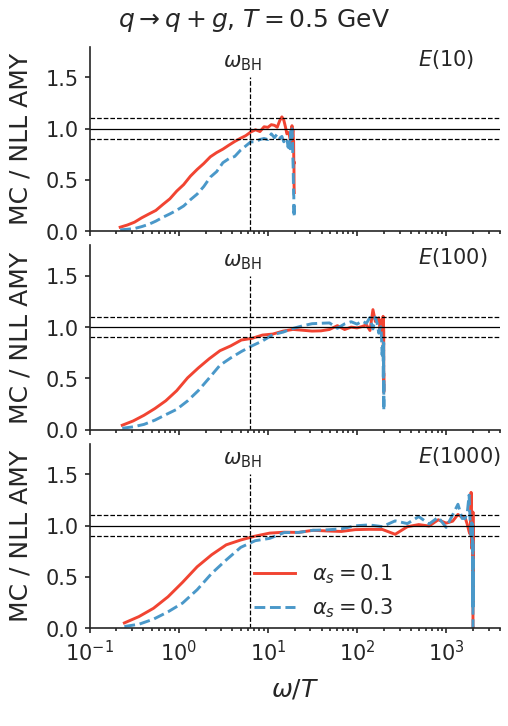
\includegraphics[width=\columnwidth]{spectrum_E_q2qg.png}
\caption{Ratios of splitting rate $dR/\omega$ between the modified Boltzmann simulation and the NLL solution for $q\rightarrow q+g$ splitting. The quark energies are $E$ is 10, 100, and 100 GeV from top to the bottom plot. 
And two coupling constants are used: $\alpha_s = 0.1$ (red solid lines) and $\alpha_s = 0.3$ (blue dashed lines).
$\omega$ stands for the gluon energy.
The horizontal dashed lines denote $\pm 10\%$ deviation from unity. }
\label{fig:q2qg}
\end{figure}

\begin{figure}
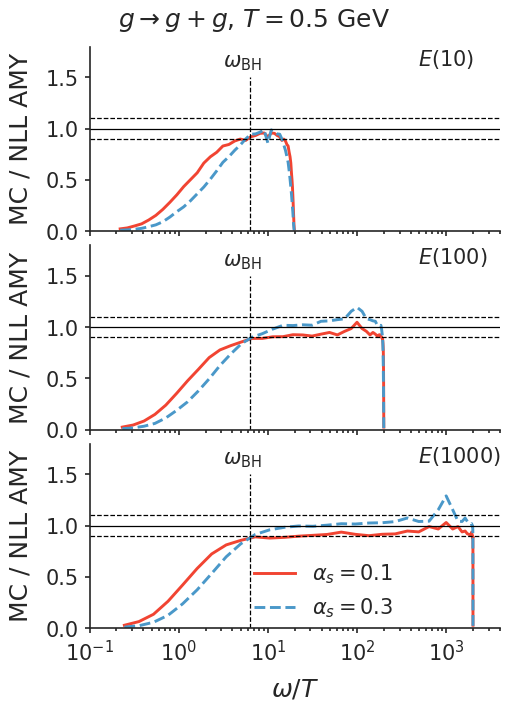
\includegraphics[width=\columnwidth]{spectrum_E_g2gg.png}
\caption{The same as Fig. \ref{fig:g2gg}, but for the $g\rightarrow g+g$ splitting, and $\omega$ stands for either energy of the final state gluon.}
\label{fig:g2gg}
\end{figure}

\begin{figure}
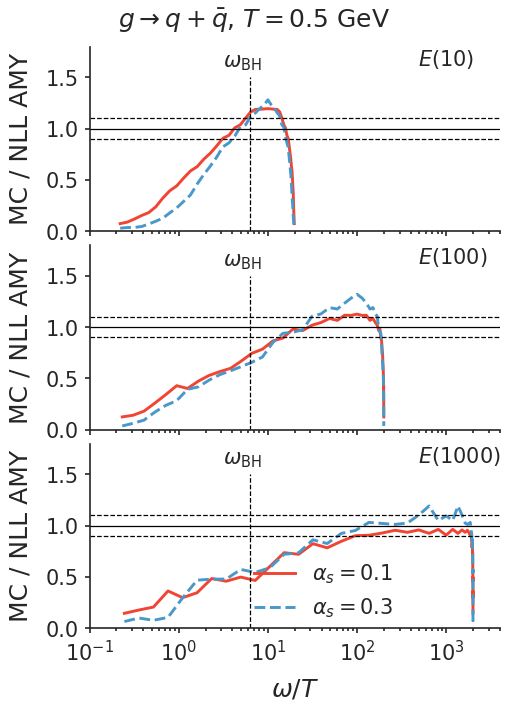
\includegraphics[width=\columnwidth]{spectrum_E_g2qqbar.png}
\caption{The same as Fig. \ref{fig:g2gg}, but for the $g\rightarrow q+\bar{q}$ splitting, and $\omega$ stands the energy of the quark.}
\label{fig:g2qqbar}
\end{figure}

\section{Energy and coupling constant dependence of the splitting rate}
In this appendix, we provide comparisons of splitting rate at different values of energy and coupling constant for the reader's references.
Fig. \ref{fig:q2qg}, Fig. \ref{fig:g2gg} and Fig. \ref{fig:g2qqbar} shows the comparison for channels $q\rightarrow q+g$, $g\rightarrow g+g$ and $g\rightarrow q+\bar{q}$ respectively.
The results are shown as the ratio between the simulations and the NLL solution.
Within in each figure, the mother parton energy are 10 GeV, 100 GeV and 1000 GeV from the top to bottom plot.
We have used two coupling constants at $\alpha_s = 0.1$ (red solid lines) and $\alpha_s = 0.3$ (blue dashed lines).

\section{Comparison of energy loss with other Monte-Carlo methods}
\label{app:tune-spectrum}
In this appendix, we compare the ``parton energy loss" from the modified Botlzmann approach to two other approaches that has been presented in the literature.
Here we have defined the so called energy loss fraction of a parton in an infinite medium as,
\begin{eqnarray}
\Delta E/E = \int x \frac{dR}{dx} dx
\end{eqnarray}
We choose to compare this quantity because the spectrum predicted in these three approaches are quite different, but it is still helpful to quantify how they differ through this way.

\paragraph{In the improved Langevin approach}
The first approach is implemented in the improved Langevin equation \cite{Cao:2013ita}, using a higher-twist calculation of  medium-induced single-gluon emission rate and a prescription to implement multiple emission in a time-evolution manner.
The higher-twist formula for single radiation rate reads,
\begin{eqnarray}
\frac{dN_g}{dx dk_\perp^2 dt} = \frac{\alpha_s P(x)\hat{q}_g}{\pi k_\perp^4} 2\left(1-\cos\frac{t-t_0}{\tau_f}\right)
\end{eqnarray}
The rate is time-dependent, coming from the interference between the production of the hard parton at time $t_0$ and one interaction with the medium at time $t$.
From the second emission, the authors of [] implements the following presciption: set the time $t_0$ to the time of the previous emission so that the probability of the next emission starts to accumulate from zero again as time increases.
Though it is not immediately clear what this prescription predicts without a simulation, it is possible to get a qualitative understanding by realizing that the typical time separation between two emissions of this model is a time scale within which the emission probability is of order one,
\begin{eqnarray}
1 \sim \int_{t_0}^{t} dt\int_{x_c}^1 dx \int dk_\perp^2 \frac{dN_g(t-t_0)}{dx dk_\perp^2 dt}
\end{eqnarray}
In the soft limit where $P(x) \sim 2/x$, $\tau_f\sim 2xE/k_\perp^2$, and perform the time integral first, then the $k_\perp$ integral with limits from $0$ to $xE$.
To render the final integral of $x$ (with a change of variable to $u = xE\Delta t/2$) finite, we need a lower cut-off of $x$ at $x_c$,
\begin{eqnarray}
1 &\sim& 4\alpha_s\hat{q}\Delta t \int_{x_c}^1 \frac{dx}{x} \int \frac{dk_\perp^2}{k_\perp^4}\left(1-\frac{\sin(\Delta t/\tau_f)}{\Delta t/\tau_f}\right)\\
&=& \frac{\alpha_s\hat{q}_g \Delta t^3}{3u^3} \left( u^3\mathrm{Ci}(u)-3u^2\mathrm{Si}(u) - u^2 \sin(u) \right. \\\nonumber
&&\left. +3u-\sin(u) - 2u\cos(u) \right) \left.\right|_{\frac{\Delta t E x_c}{2}}^{\frac{\Delta t E}{2}} 
\end{eqnarray}
The result can be expanded at small $u$: $\frac{1}{18}(6\ln(u)+6\gamma_E - 17)$, besides it decays to $0$ at infinity, so a good proxy is to use the small-$u$ expansion but cut-off the upper bound at its zero,
\begin{eqnarray}
1 &\sim&  \frac{\alpha_s\hat{q}\Delta t^3}{3}\ln\frac{2}{ x_c E \Delta t } \propto (g^2 T \Delta t)^3 \ln\frac{2}{ x_c E \Delta t }
\label{eq:delta-t-formula}
\end{eqnarray}
Now, it is clear that the typical time between two emissions in this approach is on the order of $1/g^2T$ which is the order of the elastic collision mean-free-path.
Putting typical $\Delta t \sim \lambda_{el}$ back to the factor $2(1-\cos(\Delta t/\tau_f))$, one finds that the radiation spectrum is suppressed when the formation time is much greater than the mean-free-path.
This feature certainly suppresses the energy loss relative the incoherent one, however, it is introduced by controlling the correlation between two subsequent emissions, while the LPM suppression actually happens on the level of single emission rate.
Moreover, the logarithmic factor in equation \ref{eq:delta-t-formula} depends on the infrared cut-off (in the original work, this cut-off is chosen at $\pi T$), therefore the prediction is cut-off dependent though logarithmic slow.
This is due to that this correlation prescription changes the second emission rate the same way, no matter how soft the previous emission is.
This is in fact a feature we want to avoid as the correlation between subsequent emission is a higher order question.

\paragraph{The blocking radiation approach}
Another approach that has been used before will be termed as the ``blocking radiation approach" in this work.
In this approach, the splitting is also first generated through an incoherent processes at time $t_0$, and then the self-consistent determination of formation time by elastic broadening is the same as the modified Boltzmann approach.
However, the LPM suppression is introduced by requiring no additional radiation is allowed during the formation time of the previous one.
Again, this method introduces correlations between subsequent emissions.
A closer investigation reveals bigger problem.
This approach effectively reduces every $\tau_f/\lambda_{inel}$ incoherent emission to one, resulting only an overall reduction in the radiation spectrum without changing its shape.
And the suppression factor $\lambda_{inel}/\tau_f$ is a comparison between  the formation time with the incoherent inelastic mean-free-path, instead of the elastic mean-free-path, which is off by a power of $\alpha_s$.

\begin{figure*}
\centering
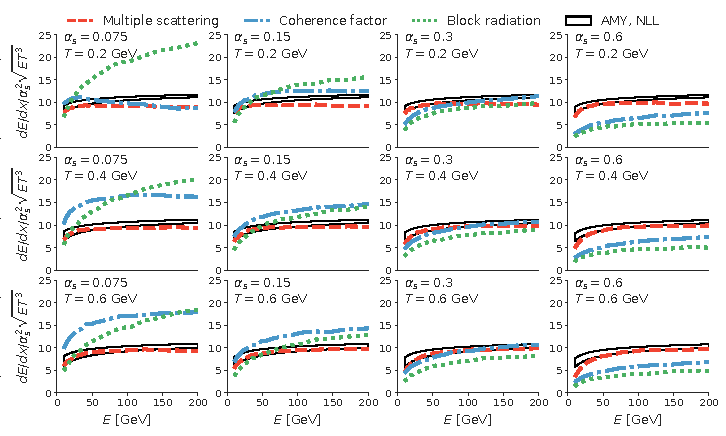
\includegraphics[width=1.\textwidth]{Eloss_infinite.pdf}
\caption{Energy loss per unit path lengh $dE/dx$ as a function of energy $E$, temperature $T$ and coupling constant $\alpha_s$. Each column corresponds to a value of the coupling constant $\alpha_s = 0.075, 0.15, 0.3$, and $0.6$ (from left to right). Each row corresponds to a temperature of $T = 0.2, 0.4$, and $0.6$ GeV (from top to bottom). $dE/dx$ is divided by the expected scaling $\alpha_s^2 \sqrt{ET^3}$. The MC implementations of the LPM effect referred to as ``modified rescattering", ``coherence factor", and ``block radiation" approaches are shown with red-dashed lines, blue-dash-dotted lines, and green-dotted lines respectively. The AMY NLL results are denoted as black boxes.}
\label{fig:eloss-inf}
\end{figure*}


\paragraph{Comparison with the modified Boltzmann approach and the analytic results}
In Figure \ref{fig:eloss-inf}, we show the calculation of energy loss per unit path length $dE/dx$ of a quark in an ``infinitely large" medium. 
The results presented are normalized by $1/(\alpha_s^2 \sqrt{ET^3})$ in anticipation of the scaling $dE/dx \propto \alpha_s^2 \sqrt{ET^3}$.
For each column, we double the value of $\alpha_s$ and for each row, the temperature is increased by $0.2$ GeV. 
Within each subplot, the parton energy varies from $10$ GeV to $200$ GeV.
The three Monte-Carlo methods of medium-induced energy loss are shown in colored lines, 
NLL AMY results are shown as black lines where we only integrate $\omega$ above the the Debye mass 
As expected, the modified Boltzmann approach (red-dashed lines) which describes the radiation spectrum also reproduces the energy, temperature, and coupling constant dependence of energy loss.
The  approach used in the improved-Langevin equation (blue-dash-dotted lines) has a similar energy and temperature dependence as the theoretical baseline; however, it systematically deviates from the baseline for different values of the coupling constant in a logarithmic manner.
For the ``block radiation" approaches, the deviations from the baseline regarding their $\alpha_s$-dependence is completely off, which is not surprising as we have discussed its shortcomings.

\end{appendices}
\bibliography{mclpm} 
\end{document}
